% Условная компиляция для самостоятельной работы
\ifdefined\mainfile
    % Если это часть основного файла, не добавляем начало и конец документа
\else
    \documentclass[12pt, a4paper]{report}
    \usepackage{/Users/vladbelousov/Desktop/Semestr_4-FP-NSU/Настройка/library}
    \usepackage[utf8]{inputenc} % Подключение поддержки UTF-8
    \begin{document}
\fi

%%-------------------------------%%


\section{Продолжение: \( E \) волна в прямоугольном волноводе }

\[ E_z \neq 0 , \text{ } B_z = 0 \] 

\[ \Delta_{ \perp  } E_z ( x,y ) + \ae ^2 E_z (x,y )= 0  \] 

\[ \text{Г.У } E_z|_{\text{Г} } = 0 \Rightarrow E_z (x,y ) = E_1 (x) E_2 (y )  \] 

\[ \underbrace{\frac{E_1 '' (x )}{E_1 (x ) }}_{-k_x ^2 } + \underbrace{\frac{ E_2 ''(y )}{E_2 (y )}}_{- k_y ^2 } + \ae ^2 = 0 \Rightarrow E_z (x,y) = E_0 \sin (k_x x + \alpha_x ) \sin (k_y y + \alpha_y)   \] 

\[ \text{Г.У } E_z |_{y= 0 , \text{ }  y = b } = 0 \Rightarrow \alpha_y = 0 , \text{ } k_y b = n_y \pi , \text{ }  E_z |_{x= 0 , \text{ } x =a  }  \Rightarrow \alpha_x = 0 , \text{ } k_x a = n_x \pi ,  \text{ } n_x ,n_y \in \mathbb{Z}  \] 

\[ E_z (\vec{r } ,  t ) = E_0 \sin (k_x x) \sin (k_y y )e^{ i k_z z - i \omega_{n_x, n_y } t } , \quad  \frac{\omega_{n_x, n_y } ^2  \varepsilon \mu}{c ^2} = k_x ^2 + k_y ^2 + k_z ^2    \] 

Мода минимальной частоты: \( E_{11}     \text{ } (n_x = 1, \text{  } n_y= 1 ) \) 

\section{ТЕМ-волны в неодносвязных волноводах }

\begin{center}
    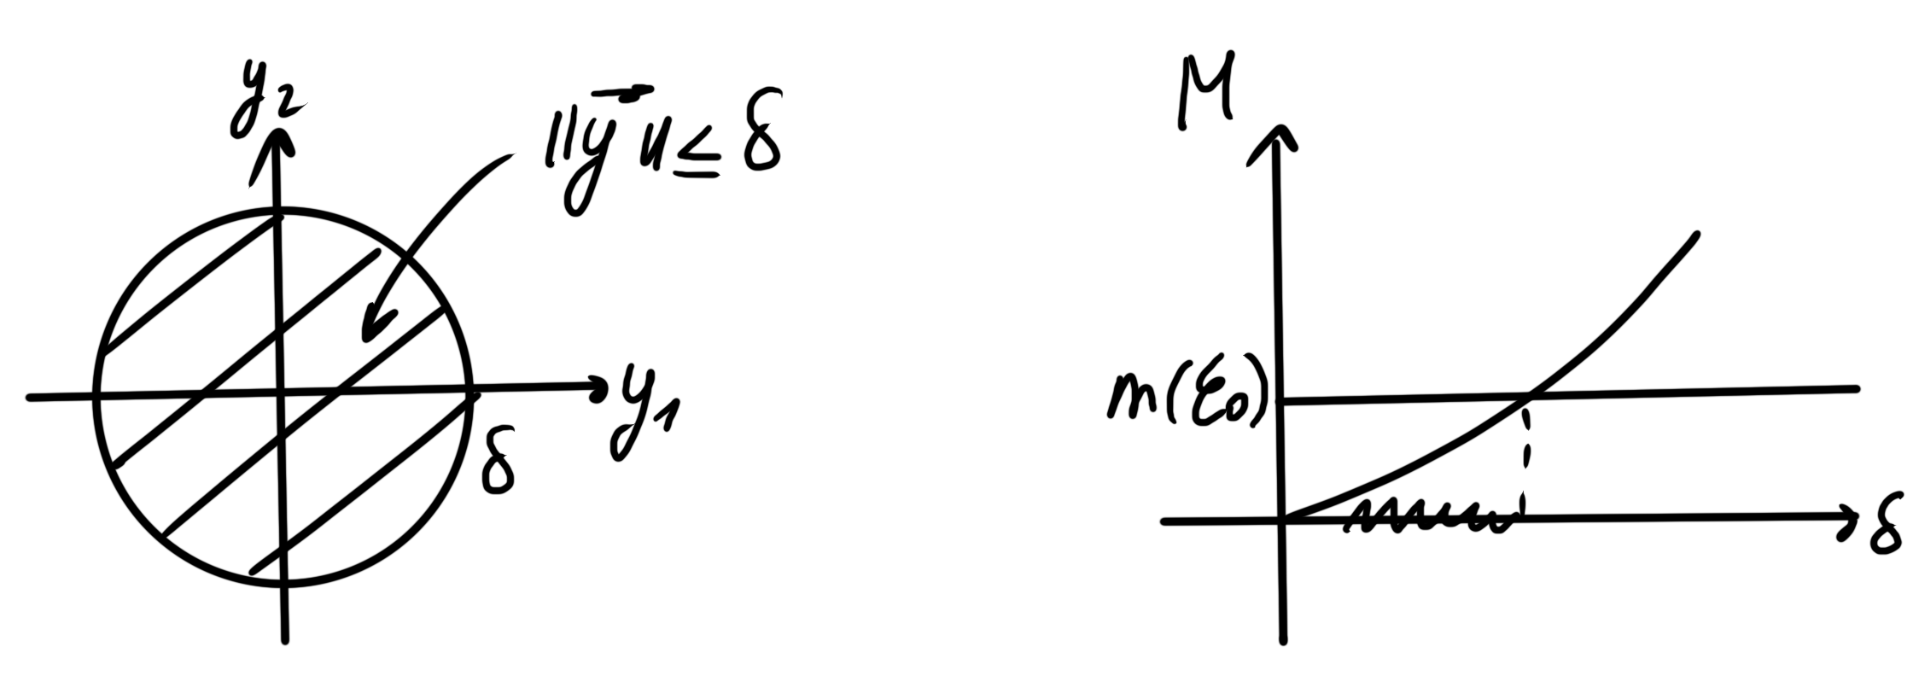
\includegraphics[width=0.3\textwidth]{/Users/vladbelousov/Desktop/Semestr_4-FP-NSU/ЭиО/Лекции_по_дням/image/59.png}
\end{center}

\begin{center}
    (1) - односвязный волновод, (2) - двухсвязный волновод;
\end{center}

В (2) помимо \( E \) и \( H  \) - волн существует ТЕМ-волна, с \( E_z = 0, \text{ } B_z = 0 \). Дисперсионное соотношение так же как для плоских монохроматических волн в свободном растворе: 

\begin{center}
    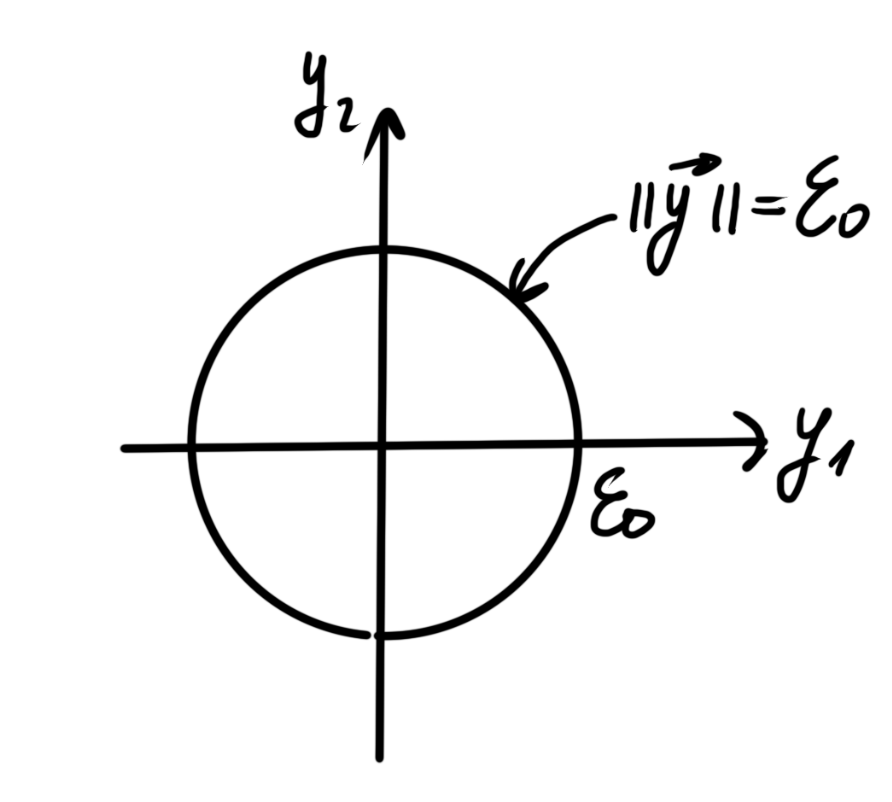
\includegraphics[width=0.3\textwidth]{/Users/vladbelousov/Desktop/Semestr_4-FP-NSU/ЭиО/Лекции_по_дням/image/58.png}
\end{center}

\begin{center}
    для случая \( \varepsilon (\omega )= \mathrm{const}, \text{ } \mu( \omega ) = \mathrm{const}     \) 
\end{center}

\[ \frac{ \omega ^2 }{c ^2 } \varepsilon \mu = k_z ^2   \]

\[ \vec{E } _{\perp  }( \vec{r }, t      ) = \vec{E } (x,y )e^{ i k_z z - i \omega t }   \] 

\[ \vec{B } _{\perp  }(\vec{r } ,t ) = \vec{B } (x,y )e^{ i k_z z - \omega t}   \] 

\[ \left( \mathrm{rot }   \vec{E }  \right)_{z }  = \frac{ i \omega }{c } (\vec{B } )_z = 0 \Rightarrow \frac{\partial  E_y } {\partial  x } - \frac{ \partial  E_x }{\partial  y} = 0 , \text{  ищем решение в таком виде:  } \vec{E} = - \nabla_{ \perp }  \varphi     \] 

\[ E_x = - \frac{\partial  \varphi }{\partial x }, \text{  } E_y = - \frac{\partial  \varphi}{\partial  y } \Rightarrow \frac{ \partial  }{\partial  x }\left( - \frac{\partial  \varphi }{\partial  y }  \right)    - \frac{ \partial  }{\partial y  }\left( - \frac{\partial  \varphi }{\partial  x }  \right) = 0 \] 

\[ \mathrm{div } \vec{E } = 0 = \frac{\partial  E_x }{\partial  x } + \frac{\partial  E_y }{\partial  y }  = \left[ \frac{\partial  ^2 \varphi }{\partial  x ^2 }+ \frac{\partial  ^2 \varphi }{\partial  y ^2 }   \right] = 0 \Rightarrow \Delta_{\perp  }  \varphi =0   \] 

Из \( E_{\tau } | _{\text{Г} }  \Rightarrow \varphi|_{\text{Г} } = \mathrm{const}     \) 

Почему в односвязном волноводе нет таких волн: 

\begin{center}
    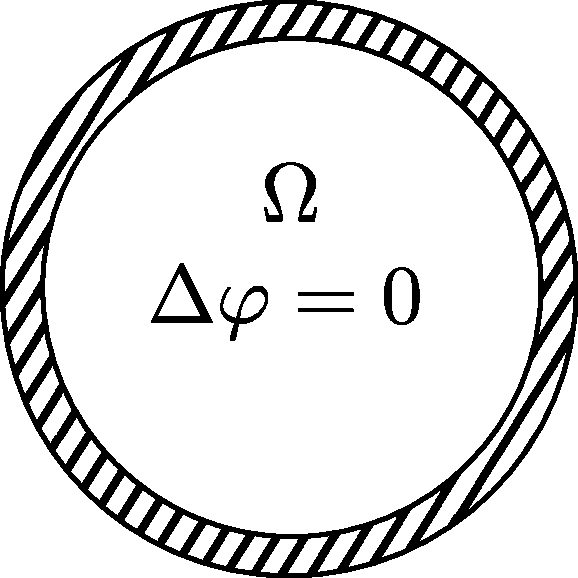
\includegraphics[width=0.2\textwidth]{/Users/vladbelousov/Desktop/Semestr_4-FP-NSU/ЭиО/Лекции_по_дням/image/60.pdf}
\end{center}

Из теоремы единственности \( \varphi     = \mathrm{const}   \) в \( \Omega  \Rightarrow - \nabla _{ \perp } \varphi = 0\) 

Для многосвязных волноводов

\begin{center}
    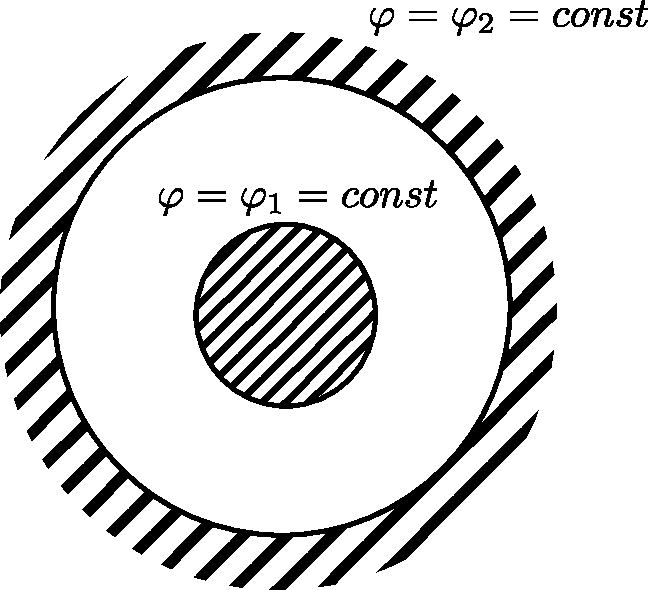
\includegraphics[width=0.3\textwidth]{/Users/vladbelousov/Desktop/Semestr_4-FP-NSU/ЭиО/Лекции_по_дням/image/61.pdf}
\end{center}

\textbf{Коаксиальный волновод (кабель):} 

\begin{center}
    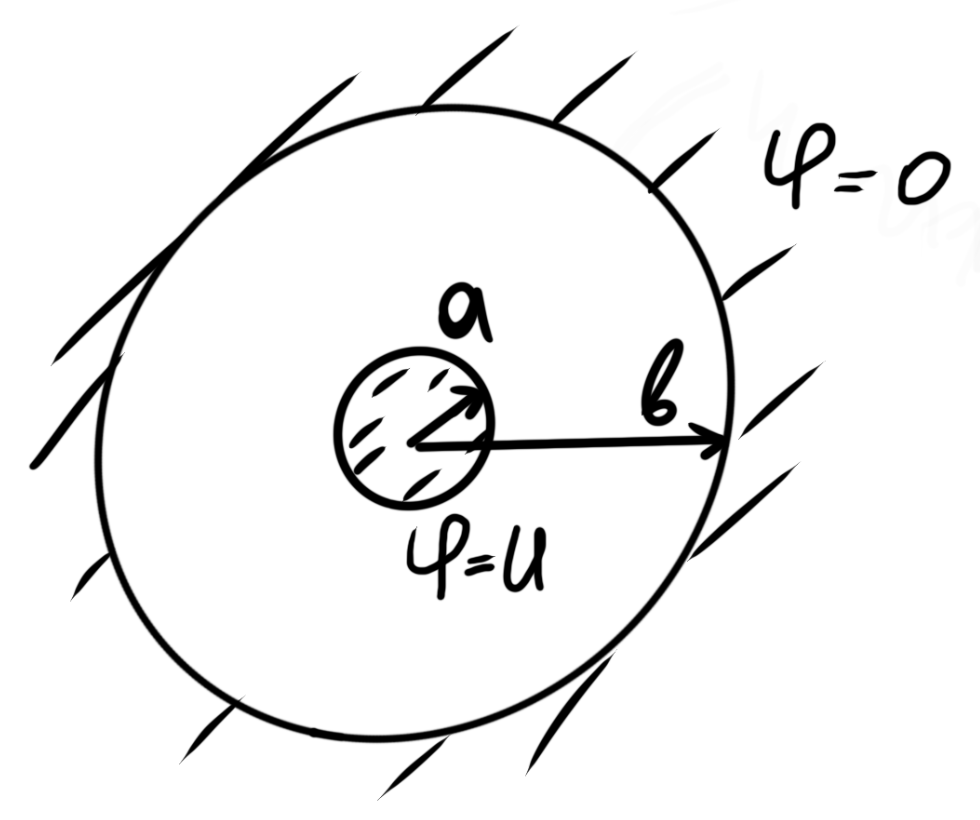
\includegraphics[width=0.3\textwidth]{/Users/vladbelousov/Desktop/Semestr_4-FP-NSU/ЭиО/Лекции_по_дням/image/61.png}
\end{center}

\[ \Delta _{ \perp  }\varphi = 0 \Rightarrow \frac{1}{r } \frac{\partial  }{\partial  r }\left(  r \frac{ \partial  \varphi }{\partial  r }  \right) + \frac{1}{r ^2 } \frac{\partial  ^2 \varphi }{\partial  \alpha ^2 }  =0   \] 

Зависимость от \( \alpha \) исключим \( \displaystyle \Rightarrow \frac{d \varphi }{dr  } =\frac{A }{r} , \text{ } A = \mathrm{const} \Rightarrow \varphi (r ) = A \ln r + B   \) 

\[ \varphi|_{r = b} =  0 ,\text{ } \varphi |_{r = b} =U \Rightarrow A \ln  b + B = 0 , \text{ } A \ln b = U \Rightarrow A = \frac{U }{\ln  \frac{a}{b} } , \text{ } B = -A \ln b   \] 

\[ \varphi(r ) = \frac{U }{\ln \frac{a}{b } } \ln \frac{r}{b }  = \frac{U }{\ln \frac{b}{a} } \ln \frac{b}{r}  , \text{ }  E_{r }  = - \frac{\partial  \varphi }{\partial  r } = \frac{U }{\ln \frac{b}{a} } \frac{1}{r}    \] 

\[ \vec{E } (\vec{r } ,t ) = \vec{e_r } \frac{U }{\ln \frac{b}{a} } \frac{1}{r} e^{i k_z z - i\omega t } ; \text{ } \vec{B } = \frac{c}{i \omega} \mathrm{rot } \vec{E } = \frac{c}{i \omega } i k_z  \frac{U }{\ln \frac{b}{a} } \frac{1}{r} e^{i k_z z - i \omega t }\vec{e } _{\alpha}   , \text{ } \frac{ \omega \sqrt{\varepsilon \mu } }{c } = k_z         \] 

\[ \vec{E } (\vec{r } ,t ) = \vec{e } _{\alpha } \sqrt{ \varepsilon \mu }  \frac{U }{\ln \frac{b}{a} } \frac{1}{r} e^{i k_z z - i \omega t }   \] 

\begin{center}
    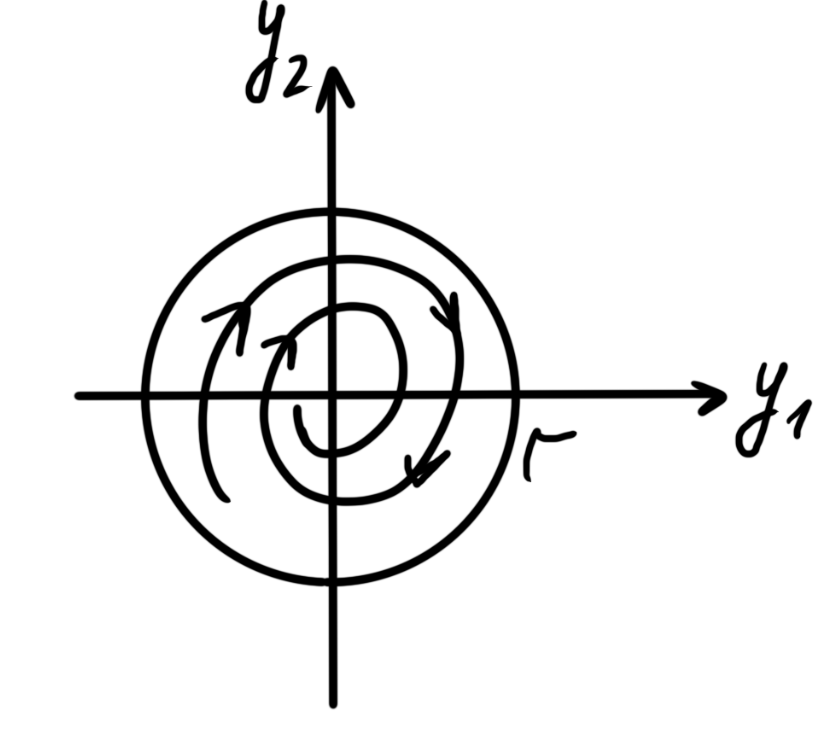
\includegraphics[width=0.3\textwidth]{/Users/vladbelousov/Desktop/Semestr_4-FP-NSU/ЭиО/Лекции_по_дням/image/62.png}
\end{center}

\section{Распространение волн в неоднородных средах}

Рассмотрим только монохроматические электромагнитные волны \( \varepsilon ( \omega , \vec{r } ) , \text{ }  \mu (\omega ,\vec{r} ) \), будем рассматривать частный случай при заданной \( \omega \Rightarrow \varepsilon (\vec{r } ), \mu ( \vec{r } ) \). 

Малый параметр \(\displaystyle  \varepsilon \sim  \frac{ \lambda\text{ - характерная длина волны} }{L \text{  - масштаб неоднородности среды}}  \ll 1   \).

Решение уравнений Максвелла для однородной системы: \( \begin{aligned}
\vec{E } (\vec{r },t     ) = \vec{E }_0  e^{i (\vec{k } ,\vec{r}) - i \omega t  }  , \text{  }  \vec{E }_0 \perp \vec{k } \\
\vec{B } (\vec{r },t     ) = \vec{B }_0  e^{i (\vec{k } ,\vec{r}) - i \omega t  }  , \text{  }  \vec{B }_0 \perp \vec{k } \\
\end{aligned} \) 


Искривления изображения в нагретом воздухе \( \Rightarrow \)  отклонение волн от прямолинейного распространения.

1) Зависимости \( \vec{E } _0  \) и \( \vec{B } _0  \) от \( \vec{r } | \)  Связь \( k \) и \( \omega \): \( \displaystyle  k ^2 = \frac{ \omega ^2 } { c ^2 }\varepsilon \mu \Rightarrow k = \frac{\omega }{c } n(\omega)   \) 

\begin{center}
    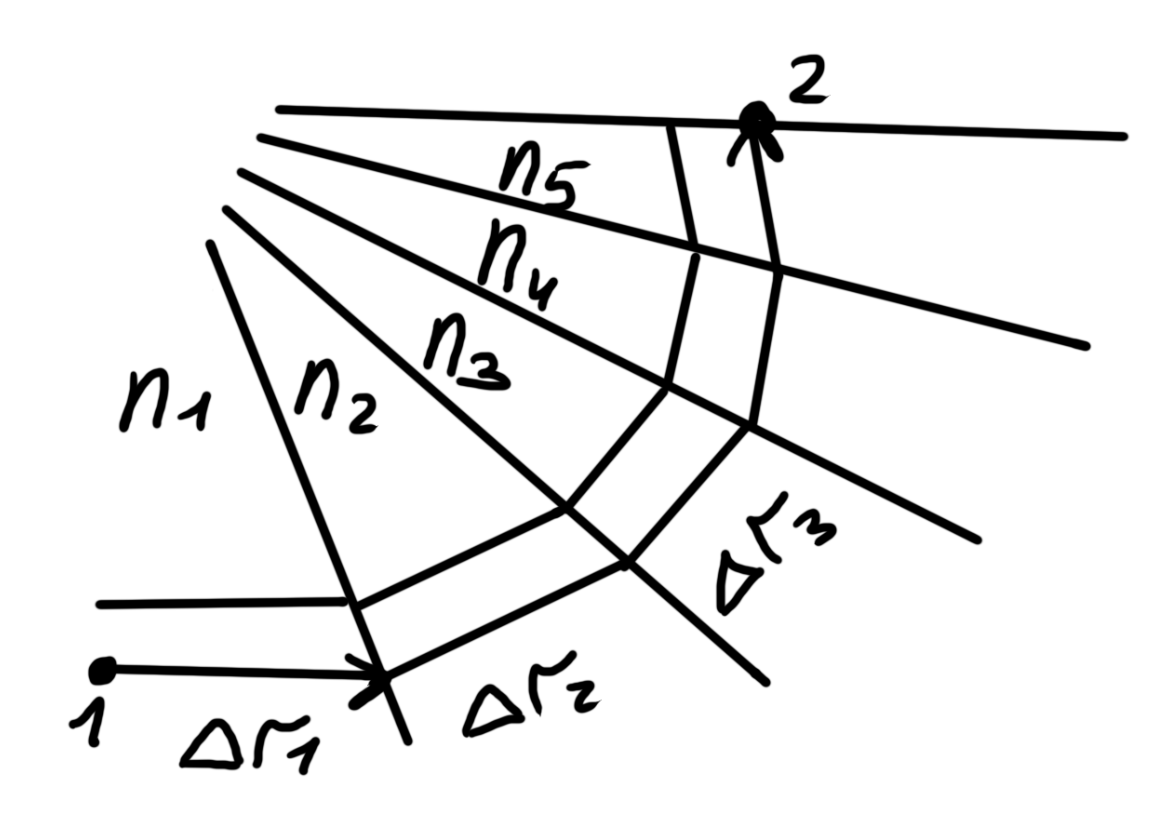
\includegraphics[width=0.3\textwidth]{/Users/vladbelousov/Desktop/Semestr_4-FP-NSU/ЭиО/Лекции_по_дням/image/63.png}
\end{center}

\[ \Delta \varphi (\text{сдвиг по фазе} ) = k_1 \Delta r_1 + k_2 \Delta r_2 +... + \sum  k_i \Delta r_i = k_0 \sum n_i \Delta r_i = k_0 \underset{\text{оптический путь} }{\int_{1 }^{2 } n(\vec{r } )ds }= \psi (\vec{r} ) -\] 

- скалярная функция \( \vec{r}  \) - эйконал.

Пусть \( \vec{E } ( \vec{r } ,t ) = \vec{E } _0  \cdot e^{ i k_0 \psi (\vec{r } ) - i \omega t}  \to  \text{ в уравнение Максвелла} \), где \( \vec{E } _0\text { медленная функция от  } \vec{r }   \),  изменяется на масштабе \( L  \).

\[ \mathrm{rot } \left[ \vec{E_0 }(\vec{r } ) e^{i k_0 \psi (\vec{r } )- i \omega t }   \right] = -\frac{1}{c} \frac{\partial  }{\partial  t } \left[ \vec{B }_0 e^{i k_0 \psi (\vec{r } )- i \omega t}   \right]   \] 

\[ \left[ \nabla \times  \vec{E } _0 ( \vec{r } ) e^{i k_0 \psi (\vec{r} )}  \right] = \frac{i \omega }{c } \vec{B } _0 (\vec{r } ) \] 

\[  e^{i k_0 \psi (\vec{r } )} e^{ i k_0 \psi (\vec{r} )} \left[ \nabla \times  \vec{E } _0 (\vec{r } ) \right] + \left[ \nabla e^{ i k_0 \psi (\vec{r } )} \times  \vec{E }  _ 0 (\vec{r} )  \right] = \frac{i \omega }{c } \vec{B } _0 (\vec{r } ) e^{i k_0 \psi (\vec{r } )} \] 

\[  e^{i k_0 \psi (\vec{r } )} \mathrm{rot } \vec{E } _0 (\vec{r } ) + e^{i k_0 \psi (\vec{r } )} i k_0 \left[ \nabla \psi (\vec{r } ) \times  \vec{E } _0 (\vec{r } ) \right] = \frac{i \omega }{c } \vec{B } _0 (\vec{r } ) e^{i k_0 \psi (\vec{r } )}    \] 

\[ \underbrace{\underset{\sim \frac{\vec{E } _0 (\vec{r } )}{L} }{\cancelto{0}{\mathrm{rot } \vec{E } _0 (\vec{r} )}} }_{E/1 \text{ см} }+ \underbrace{\underset{= \frac{2\pi}{\lambda_0} }{i k_0 }\underset{\sim 1  \vec{E } _0 (\vec{r} )}{\left[ \nabla \psi (\vec{r } ) \times \vec{E } _0 (\vec{r} ) \right] }}_{E_0/10^{-4 } \text{ см} } = \frac{ i \omega }{c }\vec{B } _ 0  (\vec{r } ) \] 

\[ \Rightarrow \left[ \nabla \psi (\vec{r } ) \times  \vec{E } _0 (\vec{r } ) \right] = \vec{B } _0 (\vec{r } ) ,\quad \mu(\vec{r } ) \mathrm{rot } \vec{H }  = - \frac{ i \omega }{c } \varepsilon (\vec{r } ) \mu (\vec{r } ) \vec{E }  \mu ( \vec{r } )  \] 

\[ \left[ \nabla \psi (\vec{r } ) \times \vec{B } _ 0 (\vec{r } )\right] = -  \varepsilon (\vec{r } ) \mu (\vec{r } ) \vec{E } _ 0 (\vec{r } ) = - n ^2 (\vec{r } ) \vec{E } _ 0 (\vec{r } ) \] 

1. \( \vec{E } _0 (\vec{r } ), \text{ } \vec{B } _0 (\vec{r } ) , \text{ }  \nabla \psi (\vec{r } ) \)  - взаимно \( \perp  \) вектора

\[ \left[ \nabla \psi \times \left[ \nabla \psi \times  \vec{E } _0 \right] \right] = - n ^2 \vec{E } _0 \] 

\[ \nabla \psi \cancelto{0}{ (\nabla \psi ,\vec{E } _0)}- \vec{E } _0 (\nabla \psi ) ^2 = - n ^2 \vec{E } _0 \] 

\[ \Rightarrow (\nabla \psi (\vec{r } )) ^2  = n ^2 (\vec{r } ) \text{ - уравнений эйконала} \] 

Как можно было бы решить это уравнение: 

\begin{center}
    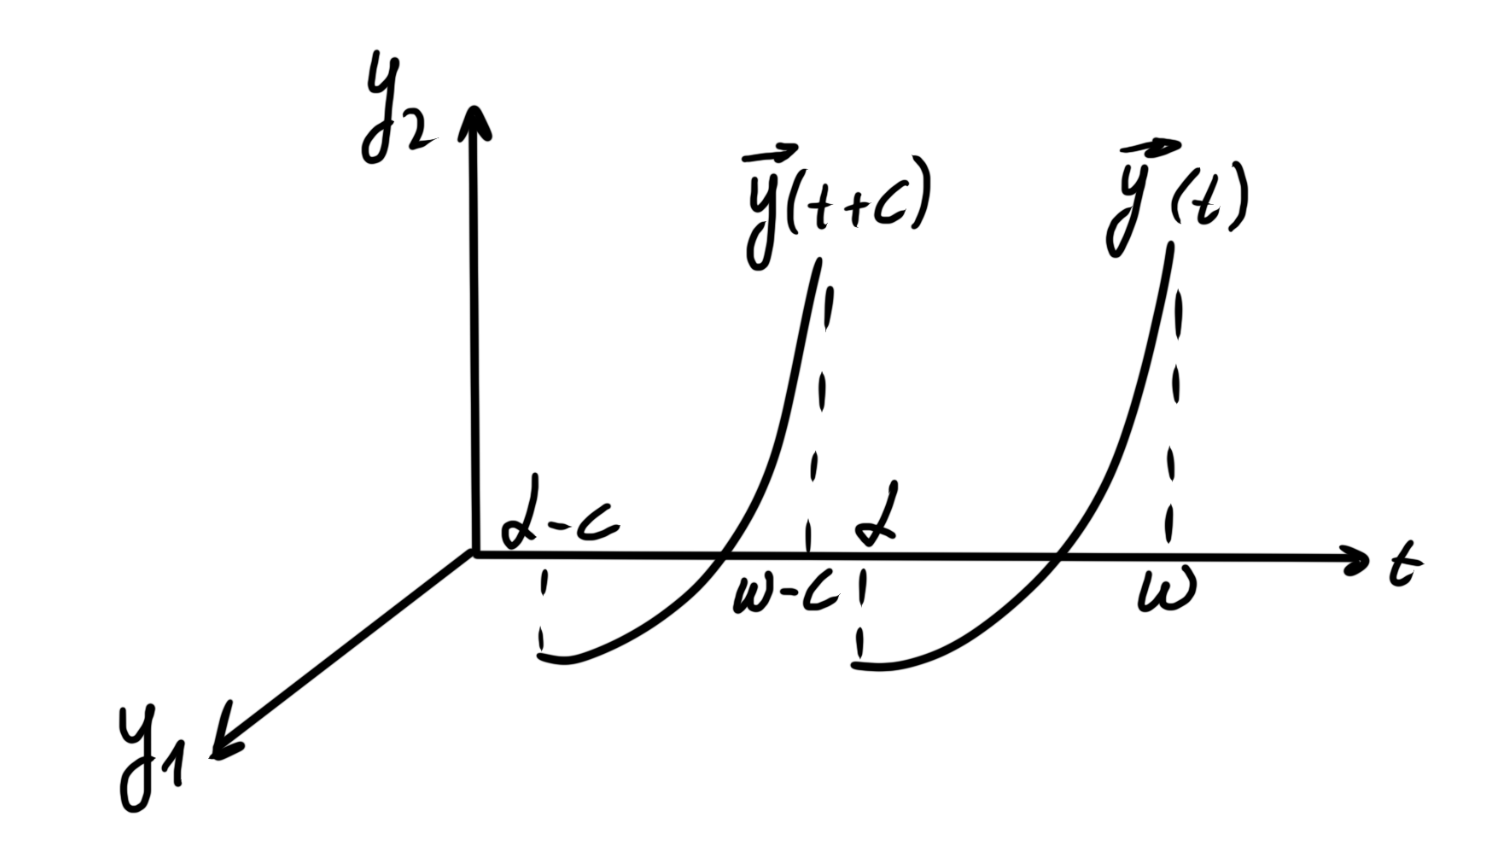
\includegraphics[width=0.5\textwidth]{/Users/vladbelousov/Desktop/Semestr_4-FP-NSU/ЭиО/Лекции_по_дням/image/64.png}
\end{center}

\[ \text{за } \Delta t \text{ }  r_{\text{волна} } = \frac{c}{n(\vec{r } )} \Delta t    \] 

(1) - волновой фронт = это поверхности \( \psi (\vec{r } ) = \mathrm{const}   \), (2) - лучи (вдоль направления \( \nabla \psi (\vec{r} ) \))/линии \( \perp  \) эквипотенциалям \( \psi (\vec{r} ) \) (волновым фронтам)

Описания распространения электромагнитной волны в неоднородных средах через волновые фронты и лучи - это два альтернативных описания. 

\[ \text{Вектор Пойнтинга: }  <\vec{\mathbb{S}} >  = \frac{c }{4 \pi } <[\mathrm{Re } \vec{E } \times  \mathrm{Re } \vec{H }   ]>  \] 

\[  <[\mathrm{Re } \vec{E } \times  \mathrm{Re } \vec{H }   ]> = <[(\vec{E } (\vec{r } )e^{ -i \omega t}  + \vec{E } ^{* } (\vec{r } )e^{ i \omega t } )] \times [\vec{H }  (\vec{r } ) e^{- i \omega t } + \vec{H } ^{* } e^{ i \omega t }  ]> = \] 

\[ \frac{ [ \vec{E } (\vec{r } ) \times  \vec{H }^* ( \vec{r } ) ]+ [ \vec{E } ^{* } (\vec{r } )\times  \vec{H } (\vec{r } )]}{4} = \frac{1}{2 }  \mathrm{Re } [\vec{E } (\vec{r } ) \times  \vec{H } ^{ * } (\vec{r} )]   \] 

\[ \vec{\mathbb{S}} = \frac{c}{8 \pi \mu } \mathrm{Re } [\vec{E } _0 (\vec{r } )\cancel{e^{ i k_0 \psi (\vec{r} )} }\times \vec{B }_0 ^{* } (\vec{r } ) \cancel{e^{- i k_0 \psi (\vec{r} )} } ]    \] 

%%-------------------------------%%

% Закрытие документа, если файл компилируется отдельно
\ifdefined\mainfile
    % Если это основной файл, не нужно заканчивать документ
\else
    \end{document}
\fi